\newcommand{\package}{\emph}

\setcounter{chapter}{1}
\setcounter{section}{0}

\section{a}

\begin{figure}[h!]
 \centering
    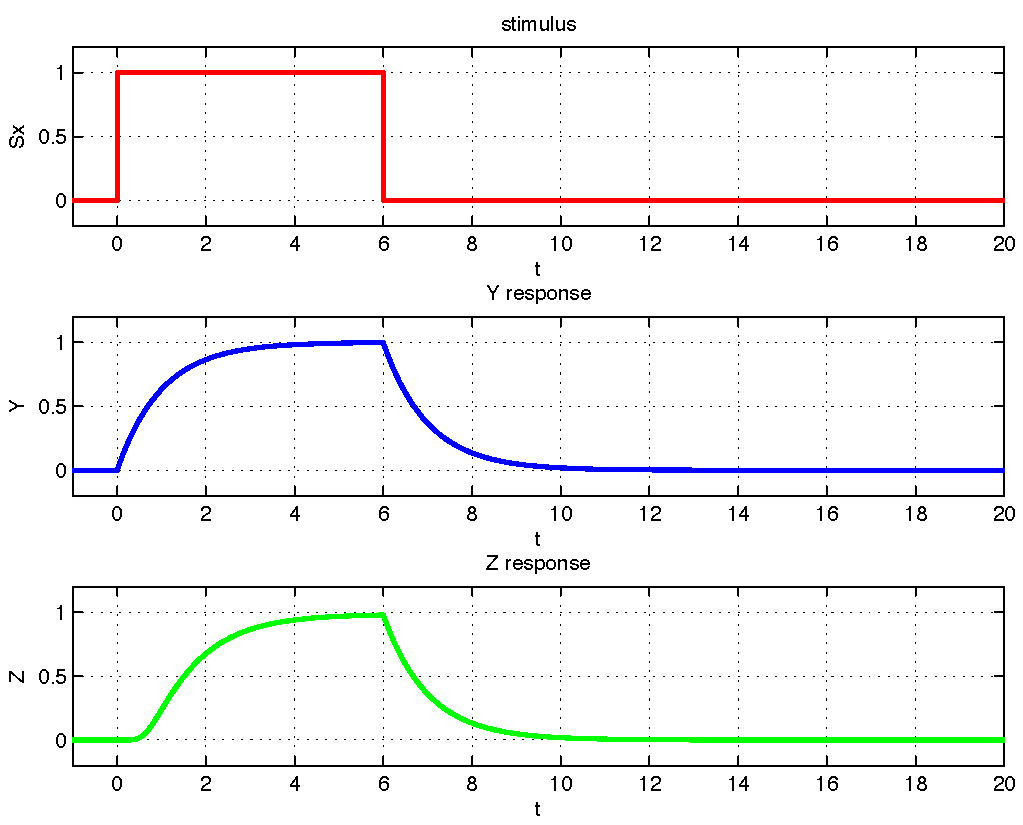
\includegraphics[scale=0.6]{plot_1A_AND} 
    \caption{Graphs illustrating system responses to the stimulus}
	\label{fig:plot_1A_AND}
\end{figure}

We report a delay in Z response after addition of the input signal \emph{$S_X$}
of $1.5200$. After the removal of the signal the concentratin on Z decreasing
immediately (no delay reported).
\newpage
\section{b}


\begin{figure}[h!]
 \centering
    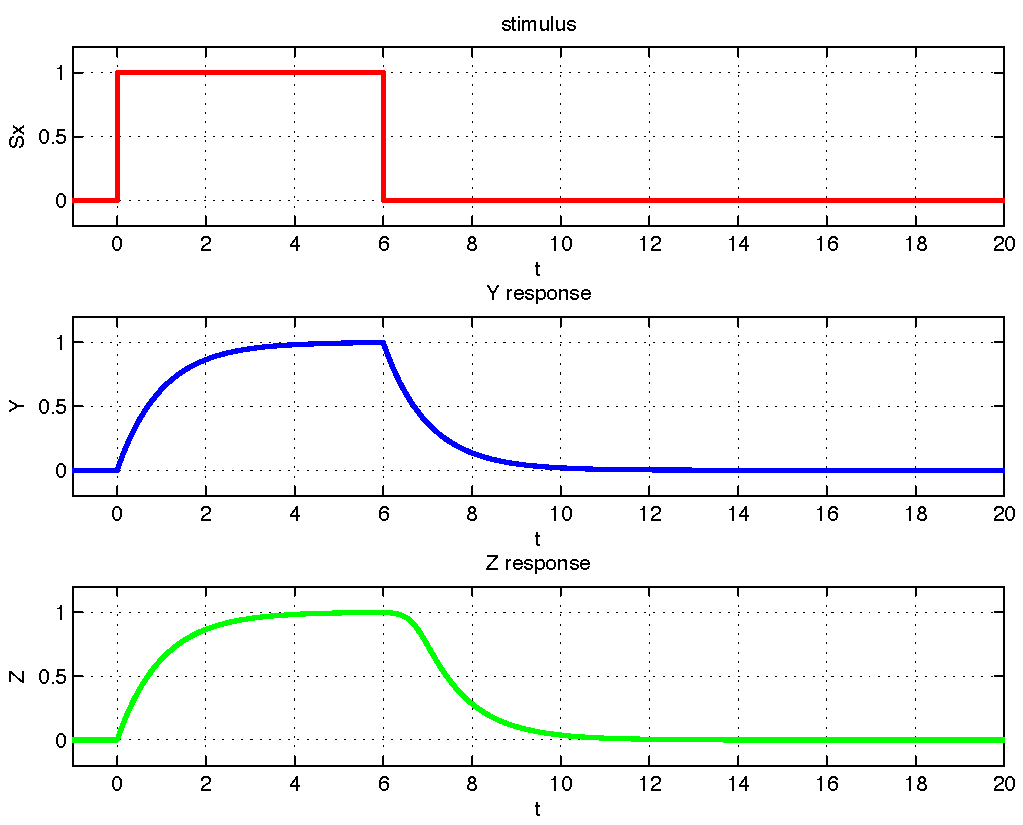
\includegraphics[scale=0.60]{plot_1B_OR} 
    \caption{Graphs illustrating system responses to the stimulus with OR
    gate and $K_{YZ} = 0.1 $}
	\label{fig:plot_1A_OR}
\end{figure}

\section{c}

\begin{table}[h!]
\begin{center}
\begin{tabular}{|l|rr|rr|r|}
\hline
Condition & Begin & End & Time begin & Time end & Duration \\
\hline
STD & $x>0$ & $x=0$ & $0.20$ & $15.88$ & $15.60$\\ 
\hline
\bottomrule
\end{tabular}
\caption{Computation of the maximum duration of the signal (STD)}
\end{center}
\end{table}			

\newpage
\section{d}

\begin{figure}[h!]
 \centering
    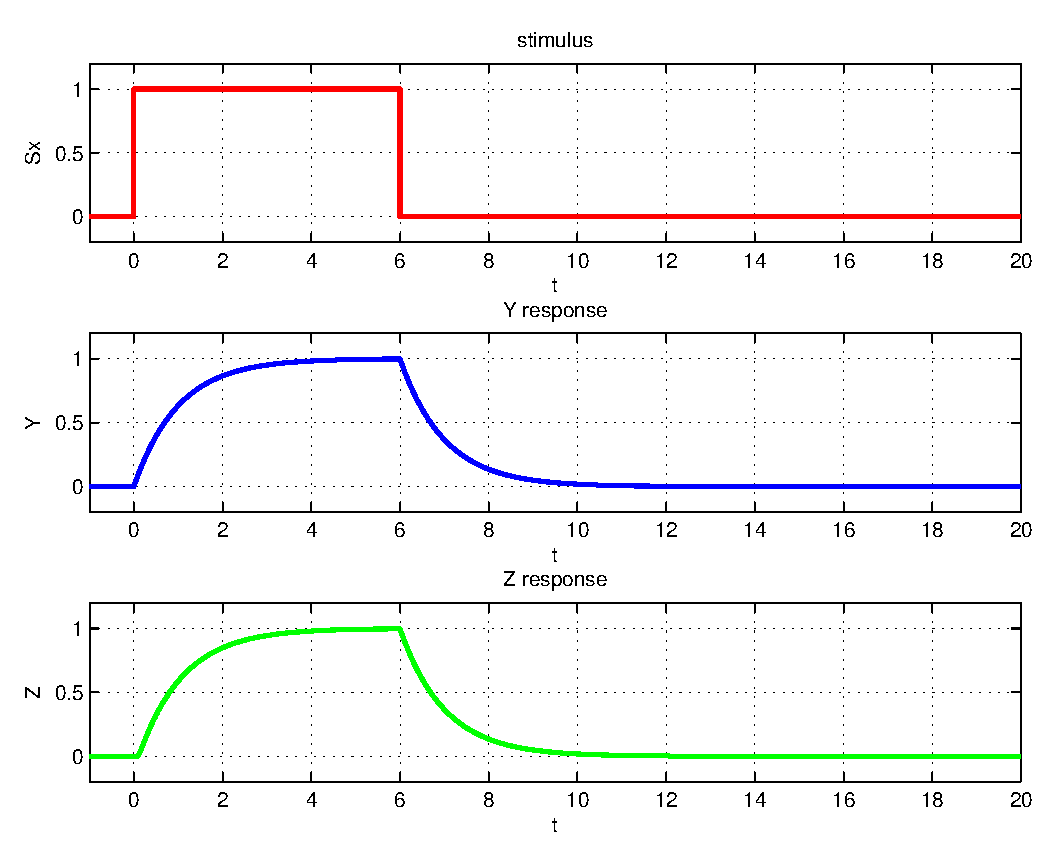
\includegraphics[scale=0.60]{plot_1D_01} 
    \caption{Graphs illustrating system responses to the stimulus with AND
    gate and $K_{YZ} = 0.1 $}
	\label{fig:plot_1D_01}
\end{figure}

\begin{figure}[h!]
 \centering
    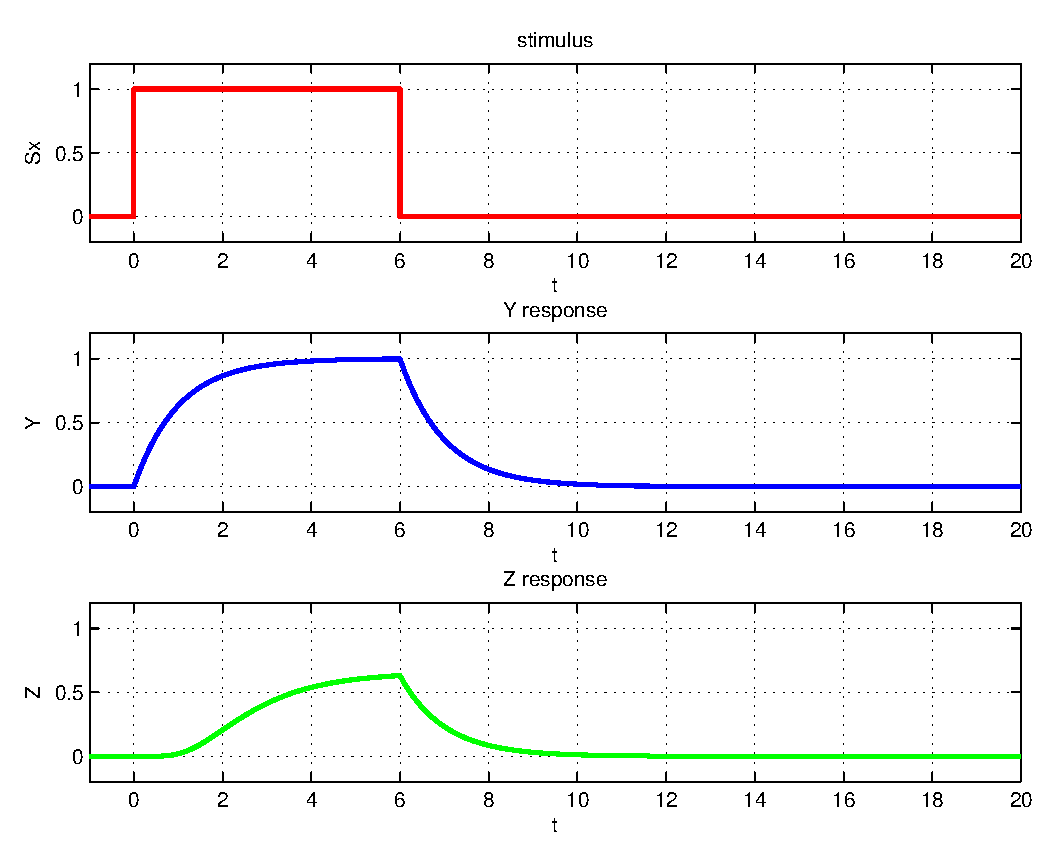
\includegraphics[scale=0.60]{plot_1D_09} 
    \caption{Graphs illustrating system responses to the stimulus with AND
    gate and $K_{YZ} = 0.9 $}
	\label{fig:plot_1D_09}
\end{figure}

\begin{table}[h!]
\begin{center}
\begin{tabular}{|l|rr|rr|r|}
\hline
Condition & Begin & End & Time begin & Time end & Duration \\
\hline
$K_{YZ} = 0.1$ & $x>0$ & $x=0$ & $0.05$ & $15.90$ & $15.85$\\ 
$K_{YZ} = 0.9$ & $x>0$ & $x=0$ & $0.34$ & $15.44$ & $15.10$\\ 
\hline
\bottomrule
\end{tabular}
\caption{Computation of the maximum duration of the signal ($K_{YZ} = 0.1$ and
$K_{YZ} = 0.9$)}
\end{center}
\end{table}	


\newpage

\setcounter{chapter}{4}
\setcounter{section}{0}

% \begin{section}{callODE.m}
% \lstinputlisting[caption={./callODE.m},label=lst:callODE-full]{./matlab_code/callODE.m}
% \end{section}
% \begin{section}{toggle.m}
% \lstinputlisting[caption={./toggle.m},label=lst:toggle-full]{./matlab_code/toggle.m}
% \end{section}
% \begin{section}{conv.m}
% \lstinputlisting[caption={./conv.m},label=lst:conv-full]{./matlab_code/conv.m}
% \end{section}
% \begin{section}{propensities.m}
% \lstinputlisting[caption={./propensities.m},label=lst:propensities-full]{./matlab_code/propensities.m}
% \end{section}
% \begin{section}{ssa.m}
% \lstinputlisting[caption={./ssa.m},label=lst:ssa-full]{./matlab_code/ssa.m}
% \end{section}
